\documentclass[11pt, oneside]{article}
\usepackage{geometry} % see geometry.pdf on how to lay out the page. There's lots.
\geometry{letterpaper} % or letter or a5paper or ... etc
% \geometry{landscape} % rotated page geometry
\usepackage{graphicx}

\usepackage{amssymb}
\usepackage{amsmath}
\usepackage{inconsolata}
% See the ``Article customise'' template for come common customisations

\title{Introduction to Programming with HERB}
\author{HERB Lab}
\date{2013-09-06} % delete this line to display the current date

%%% BEGIN DOCUMENT
\begin{document}

\maketitle


\section{Herbpy Console}
\begin{figure}[htbp]
   \centering
   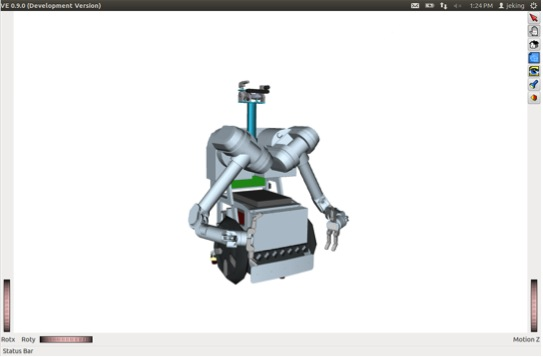
\includegraphics[width=0.8\textwidth]{figs/viewer.jpg} % requires the graphicx package
   \caption{The herbpy viewer}
   \label{fig:viewer}
\end{figure}
The easiest way to work with HERB in simulation is via the herbpy console.  To start up a herbpy console in simulation mode type the following from a command line:
\begin{figure}[h]
\centering

\includegraphics[width=0.6\textwidth]{figs/herbpystart.jpg}
\end{figure}
Here the parameter \texttt{sim} indicates you would like to start in simulation mode. The parameter \texttt{viewer} indicates that a viewer should be attached to the instance.  Figure~\ref{fig:viewer} shows an example of the viewer.  

An additional parameter that is useful is \texttt{debug}.  This will set the logging level to DEBUG.  By default, the log level is set to INFO.

Starting the herbpy console will drop into an ipython prompt.  Two useful objects have been initialized: \texttt{robot} and \texttt{env}. 

\subsection{\texttt{robot}}
The \texttt{robot} objects is a pointer to the model of the robot, in this case HERB.  Many operations on the robot are available.  The following sections outline a subset of the useful commands:

\subsubsection{Arms}\label{sec:arms}
For example, the following will give the current value of all 24 DOF values for the robot:
\begin{figure}[h]
\centering
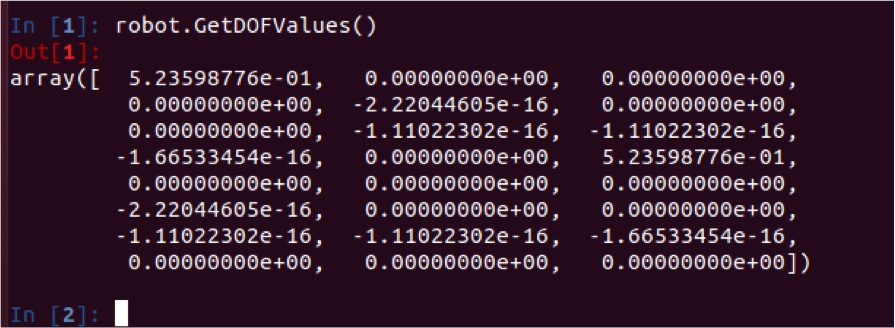
\includegraphics[width=0.8\textwidth]{figs/getdofvalues.jpg}
\end{figure}

Pointers exist for each arm of the robot via calls to \texttt{robot.left\_arm} and \texttt{robot.right\_arm}.  The following command gets DOF values for only the right arm:
\begin{figure}[h]
\centering
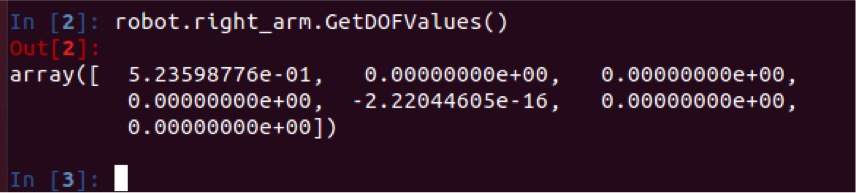
\includegraphics[width=0.8\textwidth]{figs/getrightdofvalues.jpg}
\end{figure}

Several planners exists for planning motions for the arms.  A common one, developed in this lab, is the CHOMP planner.  Prior to using the CHOMP planner, the distance field must be initialized.  The following command performs this initialization:
\begin{figure}[h]
\centering
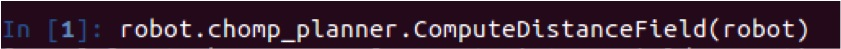
\includegraphics[width=0.8\textwidth]{figs/chompinitialize.jpg}
\end{figure}

Once this is completed, the CHOMP planner can be used to generate plans.  By default, an RRT planner is also available for planning. 

There are several methods for planning motions for arms.  The first is to plan to a pre-defined configuration.  For example the following plans the arms to the configuration seen in Figure~\ref{fig:viewer}:
\begin{figure}[h]
\centering
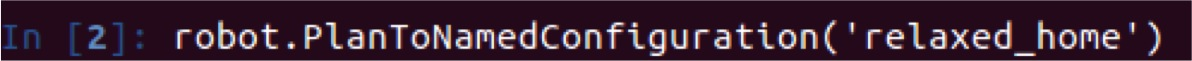
\includegraphics[width=0.8\textwidth]{figs/namedconfiguration.jpg}
\end{figure}

It is also possible to plan to a specific configuration.  For example, given the following 7 DOF configuration, \texttt{ldofs}, for the left arm:
\begin{figure}[h]
\centering
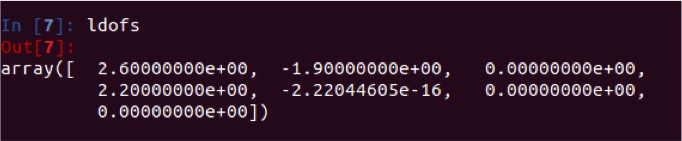
\includegraphics[width=0.8\textwidth]{figs/ldofs.jpg}
\end{figure}
\newline\newline
A plan can be generated to drive the arm to that configuration using the following:
\begin{figure}[h]
\centering
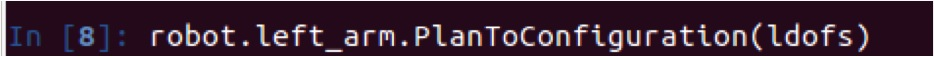
\includegraphics[width=0.8\textwidth]{figs/leftarmplanner.jpg}
\end{figure}

\newpage
\subsubsection{Hands}
In addition to the arms, the herbpy console provides hooks to actuate the hands.  For example, the following commands will open and close the right hand:
\begin{figure}[h]
\centering

\includegraphics[width=0.7\textwidth]{figs/openhand}

\includegraphics[width=0.7\textwidth]{figs/closehand}
\end{figure}

The following can be used to change the spread of the hand. Valid values are between 0 and $2\pi$:
\begin{figure}[h]
\centering
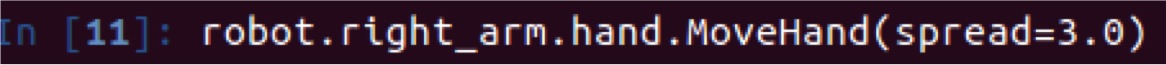
\includegraphics[width=0.8\textwidth]{figs/spread}
\end{figure}

In addition, the closure of each finger can be set individually:
\begin{figure}[h]
\centering
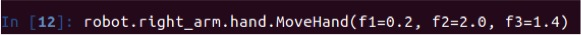
\includegraphics[width=0.8\textwidth]{figs/fingers}
\end{figure}

\newpage
\subsubsection{Base Movement}
Functions exists for moving the base of the robot.  To drive the robot forward 0.2 meters:
\begin{figure}[h]
\centering
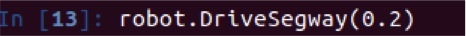
\includegraphics[width=0.6\textwidth]{figs/drivesegway}
\end{figure}
A negative input will drive the robot backwards.

Another possibly useful method for driving the base is the following:
\begin{figure}[h]
\centering
\includegraphics[width=\textwidth]{figs/drivealongvector}
\end{figure}
Here, the \texttt{direction} indicates the vector along which the robot should face.  The \texttt{goal\_pos} is the world position of the final location of the robot.  The \texttt{goal\_pos} will be projected onto the direction vector to generate a goal position for the base.

\subsection{\texttt{env}}
In addition to the \texttt{robot} object, the herbpy console is also initialized with an \texttt{env} object.  This object is a pointer to the environment in which the robot is operating.  One useful function is to add objects into that environment:
\begin{figure}[h]
\centering
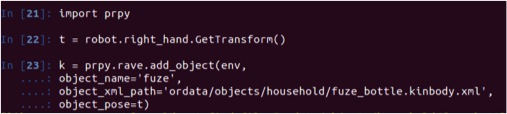
\includegraphics[width=\textwidth]{figs/addobject}
\end{figure}

The previous commands will add a model of the fuze bottle object into the environment with the same position and orientation of the right hand.  

Occasionally its useful to view a transform via drawing an axis at the appropriate position and orientation in the environment.  To do this, use the following command:
\begin{figure}[h]
\centering
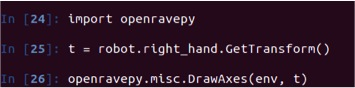
\includegraphics[width=0.7\textwidth]{figs/drawaxes}
\end{figure}

\newpage
\section{Interacting with HERB}
To interact with the real herb (not in simulation), you can start a herbpy console without the simulation flag in a window where herb is set as the rosmaster:
\begin{figure}[h]
\centering
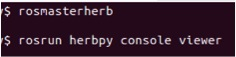
\includegraphics[width=0.4\textwidth]{figs/realherb}
\end{figure}

The model of herb in this viewer should reflect the actual configuration of the robot.  In addition, any commands issued in the ipython prompt  will be executed on the robot directly.

In addition to the arm commands presented in Section~\ref{sec:arms}, the following two commands are useful when working with the real robot. The first sets the arms to stiff.  The second command puts the arms back into gravity compensation mode:
\begin{figure}[h]
\centering
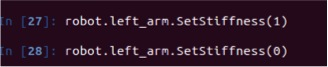
\includegraphics[width=0.6\textwidth]{figs/setstiffness}
\end{figure}

\newpage
Often it is desired to utilize the force/torque sensors in each of the wrists when working with the real robot.  To get force/torque readings:
\begin{figure}[h]
\centering

\includegraphics[width=0.6\textwidth]{figs/forcetorque}
\end{figure}

To tare the sensor:
\begin{figure}[h]
\centering
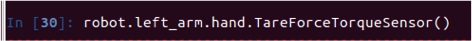
\includegraphics[width=0.6\textwidth]{figs/forcetorquetare}
\end{figure}


NOTE:  HERB is aware of only objects that are in the OpenRAVE environment.  Objects that are not present in the viewer are unknown to HERB. As a result, great care should be taken when planning in the default environment loaded by the herbpy console.

\newpage
\section{Python Scripting}
Each of the python commands shown above can be used inside a python script.  The following shows an example script that initializes a model of the robot and the environment:
\begin{figure}[h]
\centering
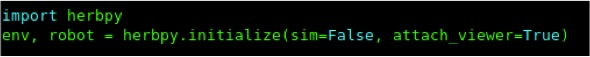
\includegraphics[width=0.6\textwidth]{figs/python}
\end{figure}
The \texttt{robot} and \texttt{env} objects are now the same as those in the herbpy console.
\end{document}